% Chapter 6

\chapter{Research Approach} % Main chapter title

\label{Chapter6_research-approach} % For referencing the chapter elsewhere, use \ref{Chapter6} 

\section{Introduction }
This chapter covers the approach taken to select the research methodology and factors considered in selecting the research methodology. After exploring different research methods in 
\citep{recker2012scientific}, 
I found that Design Science Research (DSR) methods would be the most appropriate method in this thesis. 
The detailed reasoning about the research approach 
(FIGURE \ref{fig:Research Flow})
is explained in further sections of this chapter.

\begin{figure}[ht]
    \centering
    \fbox{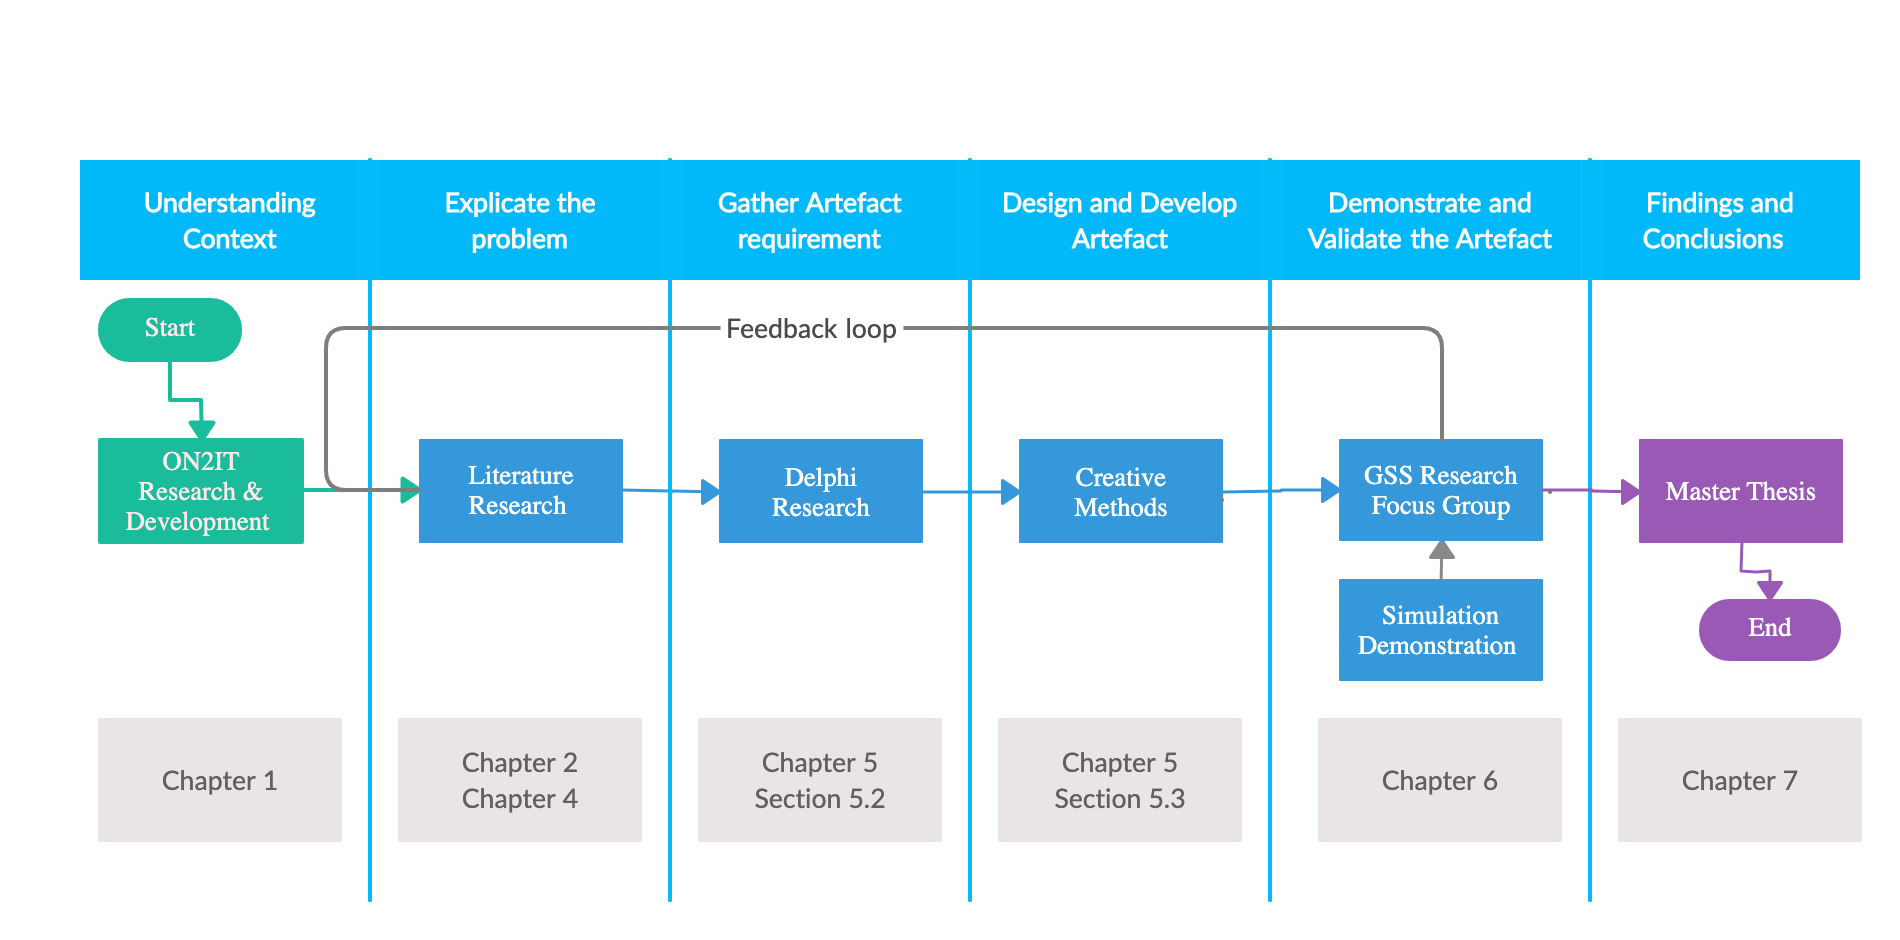
\includegraphics[width=1\linewidth]{Figures/Research Flow.png}}
    \caption{Research Approach and Structure of the thesis}
    \label{fig:Research Flow}
\end{figure}
\section{Research Methodologies } 

To determine the research methodology for the research process, 
I have examined the following four research methods:  
Quantitative, Qualitative, Mixed Methods and Design Science Research (DSR)
\citep{recker2012scientific}.

\subsection{Research Methodologies According to Scientific Research in Information Systems}

I summarize the methods as following:

\begin{enumerate}

    \item The Quantitative Methods are used to uncover truth using data collection as scientific evidence.
    
    \item The Qualitative Methods are used to explore social and cultural phenomena using texts for data interpretation.
 
    \item The Mixed Methods and used to combine both Qualitative and Quantitative for generating as well as testing the grounded theory.
    
    \item The Design Science Methods (DSR) are used to describe artificially crafted solutions for the design problems.
    
\end{enumerate}

%In an attempt to define my research methodology, I have evaluated all the four research methods proposed by the author \citeauthor{recker2012scientific}, in his book \citep{recker2012scientific}. Based on the reasoning provided by the author, I found that:
\subsection{AMS Guidelines}
I have also considered the recommendation from AMS regarding the master thesis project as depicted  in FIGURE \ref{fig:relevance-rigor}. 

\begin{figure}[ht]
    \centering
    \fbox{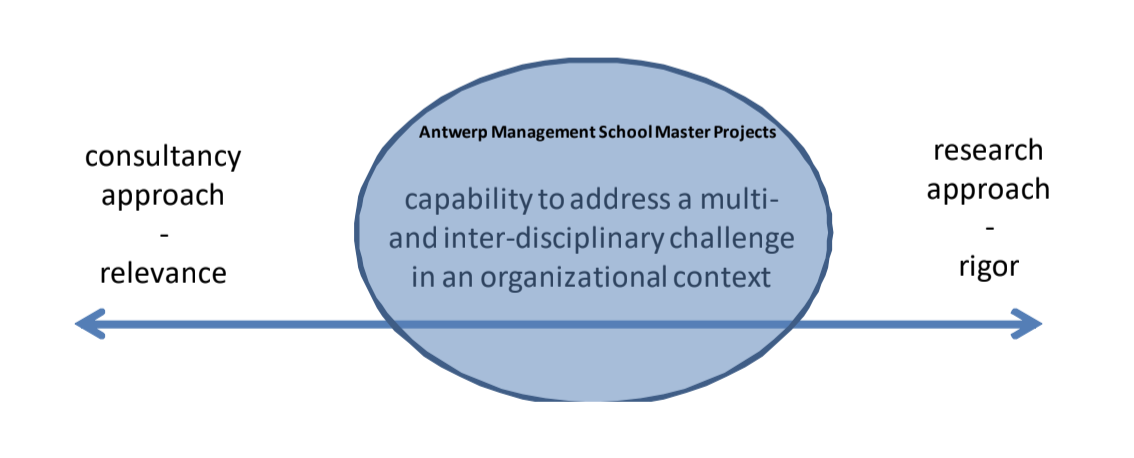
\includegraphics[width=1\linewidth]{Figures/relevance-rigor.png}}
    \caption{Balancing both rigor and relevance}
    \label{fig:relevance-rigor}
\end{figure}
\begin{quote}
`As we do adhere to
balancing both rigor and relevance, recommendations coming out of the master project should be
practical in nature and most relevant for organizations.` 
- Antwerp Management School
\end{quote}

\begin{figure}
\centering
    \includegraphics[scale=.75]{Figures/dsr.png}
    \caption{DSR  Cycle \citep[p. 80]{hevner2004design}}
    \label{fig:dsr }
\end{figure}

\section{Why Design Science Research?}
\label{Research Methodology: Design Science Research}

Since I wanted to explore methods to solve the problem at hand of absence of actionable news, 
I have chosen a research approach that does just that. First explicating the problem, 
than drafting requirements and than  establishing the prototype artefact that can be validated by the target group 
\citep{bobbert2018improving}.  
Considering the research requirements of building an artefact using rigor and relevance, 
I have concluded that it cannot be achieved  by  other methods but DSR.

\subsection{Factors consideration}

After evaluating DSR for my research which is about crafting a new artefact, 
I found that DSR Methods would guide best in the given factors of:

 \begin{enumerate}
     \item Stakeholders needs of cyber newsfeed.
     \item Building and Evaluating the Artefact.
     \item Application of existing knowledge.
     \item Balancing both rigor and relevance 
     (AMS recommendation)
     FIGURE \ref{fig:relevance-rigor}. 
 \end{enumerate}
 
\subsection{Additional consideration}

According to \cite{march1995design}, 
use of DSR methods are prominent to build and evaluate an artefact.
I would endorse my selection of using DSR methods 
to create and evaluate  Model, Method and Instantiation 
as shown is (TABLE \ref{table:research-activity}), 
where our requirements of creating an artefact 
highly resonates with the Design Science methods (DSR).

%% This file contains only a table.
%% this file is included into Chapter8

\begin{table}[bp]
   \setlength{\arrayrulewidth}{0.1mm}
    \setlength{\tabcolsep}{3pt}
    \renewcommand{\arraystretch}{1.5}

    \centering{}
 
    \caption{Research activities and outputs 
    adapted from \citep{march1995design}}
    \label{table:research-activity}
    
    \begin{tabularx}
    {\columnwidth}{|l|l|X|X|X|X|} 
    
%    |a|>{\columncolor[HTML]{FFFFFF}}C|C|C|
     \arrayrulecolor[HTML]{06000A}
        %% Table Body
       
        \hline
         \rowcolor[HTML]{FFFFFF}& & Constructs & Model & Method & Instantiation \\
        \hline
   
\cellcolor[HTML]{ECB4E8} &Build	&  	\multicolumn{1}{c|}{ \cellcolor[HTML]{ECB4E8} ---- }& \cellcolor[HTML]{ECB4E8}$X$ & \cellcolor[HTML]{ECB4E8}$X$ & \cellcolor[HTML]{ECB4E8}$X$	\\    \cline{2-2}\cline{4-6}
\multirow{-2}{*}{\cellcolor[HTML]{ECB4E8} \textbf{Design Science}} & Evaluate & 	\multicolumn{1}{c|}{ \cellcolor[HTML]{ECB4E8}----}&  \cellcolor[HTML]{ECB4E8}$X$ & \cellcolor[HTML]{ECB4E8}$X$ & \cellcolor[HTML]{ECB4E8}$X$
		\\  \hline 

\cellcolor[HTML]{BFCEED} &Theorize	& 	\multicolumn{4}{c|}{ \cellcolor[HTML]{BFCEED} --Not Applicable--}	\\  \cline{2-2}
\multirow{-2}{*}{\cellcolor[HTML]{BFCEED} \textbf{Natural Science}} & Justify & 	\multicolumn{4}{c|}{ \cellcolor[HTML]{BFCEED}--Not Applicable--}	\\   \hline


    \end{tabularx}

\end{table}








 \FloatBarrier

\section{Design Science Research Components}

Literature review, Delphi research, Creative process and 
GSS research are the DSR components applied in this research work.
I have explored the paper
\citep{bobbert2017defining} and  
\citep{bobbert2017exploring}. 
In these papers, the author has examined different research methods for designing and engineering an artefact. 
\cite{bobbert2017exploring} states that 
Design Science Research (DSR) (FIGURE \ref{fig:dsr }) 
Strategy advocates triangulation of different research methods 
within DSR to be applied during multiple research phases. 
Different research methods used during this research are listed below. 

\begin{enumerate}
    \item To explicate the problem: 
    I have used Literature Research to gain insight on the existing work on cyber newsfeed related work according to academic literature. Further, to gather the requirements from users, in this case cyber analysts.
    
    \item To gather requirements: 
    I have used Delphi Research methods
    \citep{linstone1975delphi}, ON2IT agile ceremonial events like: stand-ups(twice a week), short calls, multiple meetings with the team and exclusive individual interactions were planned to collect and refine the requirements.
    
    \item To design and develop the prototype: 
    Creative Process
    \citep{mednick1962associative} 
    was used.
    
    \item To demonstrate and validate the prototype: 
    Group Support System (GSS) research for validating the artefact 
    in order to execute DSR since validating is hard and complex 
    \citep{arnott2010relevant}. 
    For validation we planned to took an overall perspectives and experiences of the Strategic, Tactical and Organizational level
    \citep{Bobbert-Y-2019} functions or stakeholders. 
    The group (six to eight) would discuss on specific topics and the questions would be designed for free expression.
   
\end{enumerate}
 If I am looking at the combinations in the DSR, I am using multiple research applied by \cite{bobbert2017exploring} for an artefact creation as shown TABLE \ref{table:GSS}.


%% This file contains only a table.
%% this file is included into Chapter8

\begin{table}[ht]
    \setlength{\arrayrulewidth}{0.1mm}
    \setlength{\tabcolsep}{4pt}
    \renewcommand{\arraystretch}{1.0}
    
    \centering{}
    
    \caption{GSS Contribution in BIS Artefact adapted from \citep{bobbert2017exploring}}
    \label{table:GSS}
    
    \begin{tabularx}{0.96\linewidth}{|>{\columncolor[HTML]{ECB4E8}} p{1.5cm}|p{11.55cm}|} 
    
%    |a|>{\columncolor[HTML]{FFFFFF}}C|C|C|
    \arrayrulecolor[HTML]{06000A}
    
        %% Table Body
        \hline
       
         \rowcolor[HTML]{BFCEED}     
         \textbf{Type of research within DSR} 
         & 
         \textbf{Contribution to designing and engineering a Business Information Security artefact}
         \\
        \hline
        Literature research 
        &
        Explicating and defining the problem in a systematic, structured way. Objectivity removes the
        element of Fear Uncertainty and Doubt (FUD). Unbiased, structured point of departure for the
        design cycle. Requires a certain level of expertise in the topic.
         \\
        \hline
        Delphi research
        &
        Anonymous inventory and selection of views and standpoints (preferably based upon
literature data). Rigorous examination process for scrutinizing the problem via, for example,
expert opinions. Collecting global views on criteria requirements with the use of technology.
Knowledge sharing. Enables double loop learning via multiple iterations. Automated. No
geographical limitations. Limited in group interaction and discussion.
         \\
        \hline
        Group Support System research 
        & 
        Enables to create, share and capture knowledge as well as design items.
        Stimulates design thinking and stakeholder collaboration due to the “group element”. 
        Ability to collect, assess and select product requirements in a very short time frame. 
        Supports the regulative process of testing and validating requirements. 
        Processing large data sets.
        Double Loop learning. 
        Bridging knowing-doing gaps. 
        Stimulating group dialogues (i.e. among Boards of Directors and Management teams).
        Makes it possible to establish group consensus. 
        Supports the decision making process. 
        Threat of the “law of the decibel”. 
        Requires professional group moderation skills.  	
        \\
       \hline
    \end{tabularx}

\end{table}









 \FloatBarrier



\section{Research Flow}
In FIGURE \ref{fig:Research Flow}, the research flow and related research work with the link to the Chapters in this book can be visualised.

 

%---------removed pic, used tab----
%\begin{figure}
%\centering
%    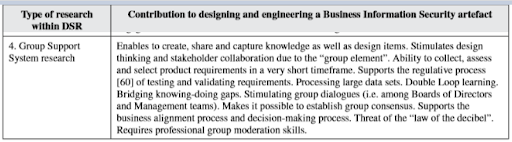
\includegraphics[scale=0.60]{Figur%es/GSS.png}
%    \caption{GSS contribution in BIS %Artefact }
%    \label{fig:GSS }
%\end{figure}
%---------removed pic, used tab----
\section{Conclusion}

Thus, along with the DSR framework, Literature review, Delphi research, Creative process and 
GSS research methods  are used to create requirements,
demonstrate and validate the  artefact's first version.
 
